% This LaTeX was auto-generated from MATLAB code.
% To make changes, update the MATLAB code and export to LaTeX again.

\documentclass{article}

\usepackage[utf8]{inputenc}
\usepackage[T1]{fontenc}
\usepackage{lmodern}
\usepackage{graphicx}
\usepackage{color}
\usepackage{hyperref}
\usepackage{amsmath}
\usepackage{amsfonts}
\usepackage{epstopdf}
\usepackage[table]{xcolor}
\usepackage{matlab}

\sloppy
\epstopdfsetup{outdir=./}
\graphicspath{ {./submission_images/} }

\matlabmultipletitles

\begin{document}

\matlabtitle{ECE1150 ASSIGNMENT6}

\begin{par}
\begin{flushleft}
Yinhao Qian @ University of Pittsburgh
\end{flushleft}
\end{par}

\begin{matlabcode}
%please ignore this block
answer = @(num,unit) fprintf("<strong> ANSWER: %s [%s]" + ...
    " </strong>\n",mat2str(num),unit);
question = @() eval("clearvars -except answer question");
\end{matlabcode}


\matlabtitle{P1-A}

\begin{par}
\begin{flushleft}
Preamble: allows receiver to differentiate actual packet from noise and sync with sender.
\end{flushleft}
\end{par}

\begin{par}
\begin{flushleft}
SFD: indicates start of frame.
\end{flushleft}
\end{par}

\begin{par}
\begin{flushleft}
Source and Destination Address: contains the MAC address of source and destination,
\end{flushleft}
\end{par}

\begin{par}
\begin{flushleft}
Length: number of bytes it gets after sfd and last four bytes are taken for CRC if less than 1518, and types of packets if greater than 1518.
\end{flushleft}
\end{par}

\begin{par}
\begin{flushleft}
Data: typically IP packets.
\end{flushleft}
\end{par}

\begin{par}
\begin{flushleft}
FCS: 32 bits CRC value, aka the frame check sequence.
\end{flushleft}
\end{par}

\matlabtitle{P1-B}

\begin{par}
\begin{flushleft}
the Medium Access Control is 48 bits in length, and all 1's address is predefined to be the broadcast address on the local area network. The first 24 bits are organizationally unique identifiers assigned byu the IEEE, and the second 24 bits are assigned by the manufacturer for each network interface card.
\end{flushleft}
\end{par}

\matlabtitle{P1-C}

\begin{par}
\begin{flushleft}
The binary exponential backoff says if a frame experiences m collisions, a node choose value k at random from the set \{0,1,2,3,...,2\textasciicircum{}m-1\}, which means as frame experience more collisions the larger the interval from which k is chosen. It is necessary because the backoff helps enforce fair distribution of access to network resources and reduce network congestions. 
\end{flushleft}
\end{par}

\matlabtitle{P1-D}

\begin{matlabcode}
question();
m = 5;
set = 0:1:2^m-1;
ave = sum(set)/size(set,2);
answer(ave,"");
\end{matlabcode}
\begin{matlaboutput}
 ANSWER: 15.5 [] 
\end{matlaboutput}

\matlabtitle{P1-E}

\begin{matlabcode}
question();
m = 6;
set = 0:1:2^m-1;
ave = sum(set)/size(set,2);
answer(ave,"");
\end{matlabcode}
\begin{matlaboutput}
 ANSWER: 31.5 [] 
\end{matlaboutput}


\matlabtitle{P2-A}

\begin{matlabcode}
question();
table_main = containers.Map();
table_main('B')='1';
table_main('E')='2';
table_main('H')='3';
disp([table_main.keys',table_main.values']);
\end{matlabcode}
\begin{matlaboutput}
    {'B'}    {'1'}
    {'E'}    {'2'}
    {'H'}    {'3'}
\end{matlaboutput}

\begin{par}
\begin{flushleft}
Please refer to the function definitions at the end of file:
\end{flushleft}
\end{par}

\begin{par}
\begin{flushleft}
The switch works like a cache. It saves the source MAC address and corresponding interface in table if not there. The switch then reads the desitnation MAC address. 
\end{flushleft}
\end{par}

\begin{par}
\begin{flushleft}
If found, foward the frame to the corresponding interface. If not found, broadcasts frame to all devices like a hub.
\end{flushleft}
\end{par}

\begin{par}
\begin{flushleft}
Transmitting A to G:
\end{flushleft}
\end{par}

\begin{matlabcode}
table_main = transmit('G','3',table_main);
\end{matlabcode}
\begin{matlaboutput}
Cache miss from table, create pair {G,3}.
    {'B'}    {'1'}
    {'E'}    {'2'}
    {'G'}    {'3'}
    {'H'}    {'3'}
\end{matlaboutput}

\begin{par}
\begin{flushleft}
Transmitting G to A:
\end{flushleft}
\end{par}

\begin{matlabcode}
table_main = transmit('A','1',table_main);
\end{matlabcode}
\begin{matlaboutput}
Cache miss from table, create pair {A,1}.
    {'A'}    {'1'}
    {'B'}    {'1'}
    {'E'}    {'2'}
    {'G'}    {'3'}
    {'H'}    {'3'}
\end{matlaboutput}

\matlabtitle{P2-B}

\begin{matlabcode}
question();
table_main = containers.Map();
table_x = containers.Map();
table_y = containers.Map();
table_z = containers.Map();
table_main('B')='x1';
table_main('E')='y1';
table_main('H')='z1';
disp([table_main.keys',table_main.values']);
\end{matlabcode}
\begin{matlaboutput}
    {'B'}    {'x1'}
    {'E'}    {'y1'}
    {'H'}    {'z1'}
\end{matlaboutput}
\begin{matlabcode}
table_main = transmit('G','z1',table_main);
\end{matlabcode}
\begin{matlaboutput}
Cache miss from table, create pair {G,z1}.
    {'B'}    {'x1'}
    {'E'}    {'y1'}
    {'G'}    {'z1'}
    {'H'}    {'z1'}
\end{matlaboutput}
\begin{matlabcode}
table_z = transmit('G','z2',table_z);
\end{matlabcode}
\begin{matlaboutput}
Cache miss from table, create pair {G,z2}.
    {'G'}    {'z2'}
\end{matlaboutput}
\begin{matlabcode}
table_main = transmit('A','x1',table_main);
\end{matlabcode}
\begin{matlaboutput}
Cache miss from table, create pair {A,x1}.
    {'A'}    {'x1'}
    {'B'}    {'x1'}
    {'E'}    {'y1'}
    {'G'}    {'z1'}
    {'H'}    {'z1'}
\end{matlaboutput}
\begin{matlabcode}
table_x = transmit('A','x2',table_x);
\end{matlabcode}
\begin{matlaboutput}
Cache miss from table, create pair {A,x2}.
    {'A'}    {'x2'}
\end{matlaboutput}

\begin{par}
\begin{flushleft}
The above is simply repeating the steps in part (a), now let's transmit from A to G again:
\end{flushleft}
\end{par}

\begin{matlabcode}
table_main = transmit('G','z1',table_main);
\end{matlabcode}
\begin{matlaboutput}
Cache hit from table.
    {'A'}    {'x1'}
    {'B'}    {'x1'}
    {'E'}    {'y1'}
    {'G'}    {'z1'}
    {'H'}    {'z1'}
\end{matlaboutput}
\begin{matlabcode}
table_z = transmit('G','z2',table_z);
\end{matlabcode}
\begin{matlaboutput}
Cache hit from table.
    {'G'}    {'z2'}
\end{matlaboutput}

\begin{par}
\begin{flushleft}
Table Y is unused. 
\end{flushleft}
\end{par}


\matlabtitle{P3-A}

\begin{par}
\begin{flushleft}
CSMA/CA DCF stands for Distributed Coordination Function. It waits for a period of time called DIFS, transmit if channel is still idle, then wait for ACK (similar to stop-and-wait ARQ).
\end{flushleft}
\end{par}

\begin{par}
\begin{flushleft}
CSMA/CA PCF stands for Point Coordination Function. Device wishing to transmit first sends Request To Send (RTS) to the AP, specifiying the duration of the requested transmittion. If no other device is tranmitting, the AP replies with Clear to Send (CTS) specifying the duration. All devices hear the CTS and will not transmit.
\end{flushleft}
\end{par}

\matlabtitle{P3-B}

\begin{matlabcode}
openExample('comm/ALOHAAndCSMACAPacketizedNetworkExample');
\end{matlabcode}

\matlabtitle{P3-C-1}

\begin{par}
\begin{flushleft}
Using the ALOHA model:
\end{flushleft}
\end{par}

\begin{par}
\begin{flushleft}
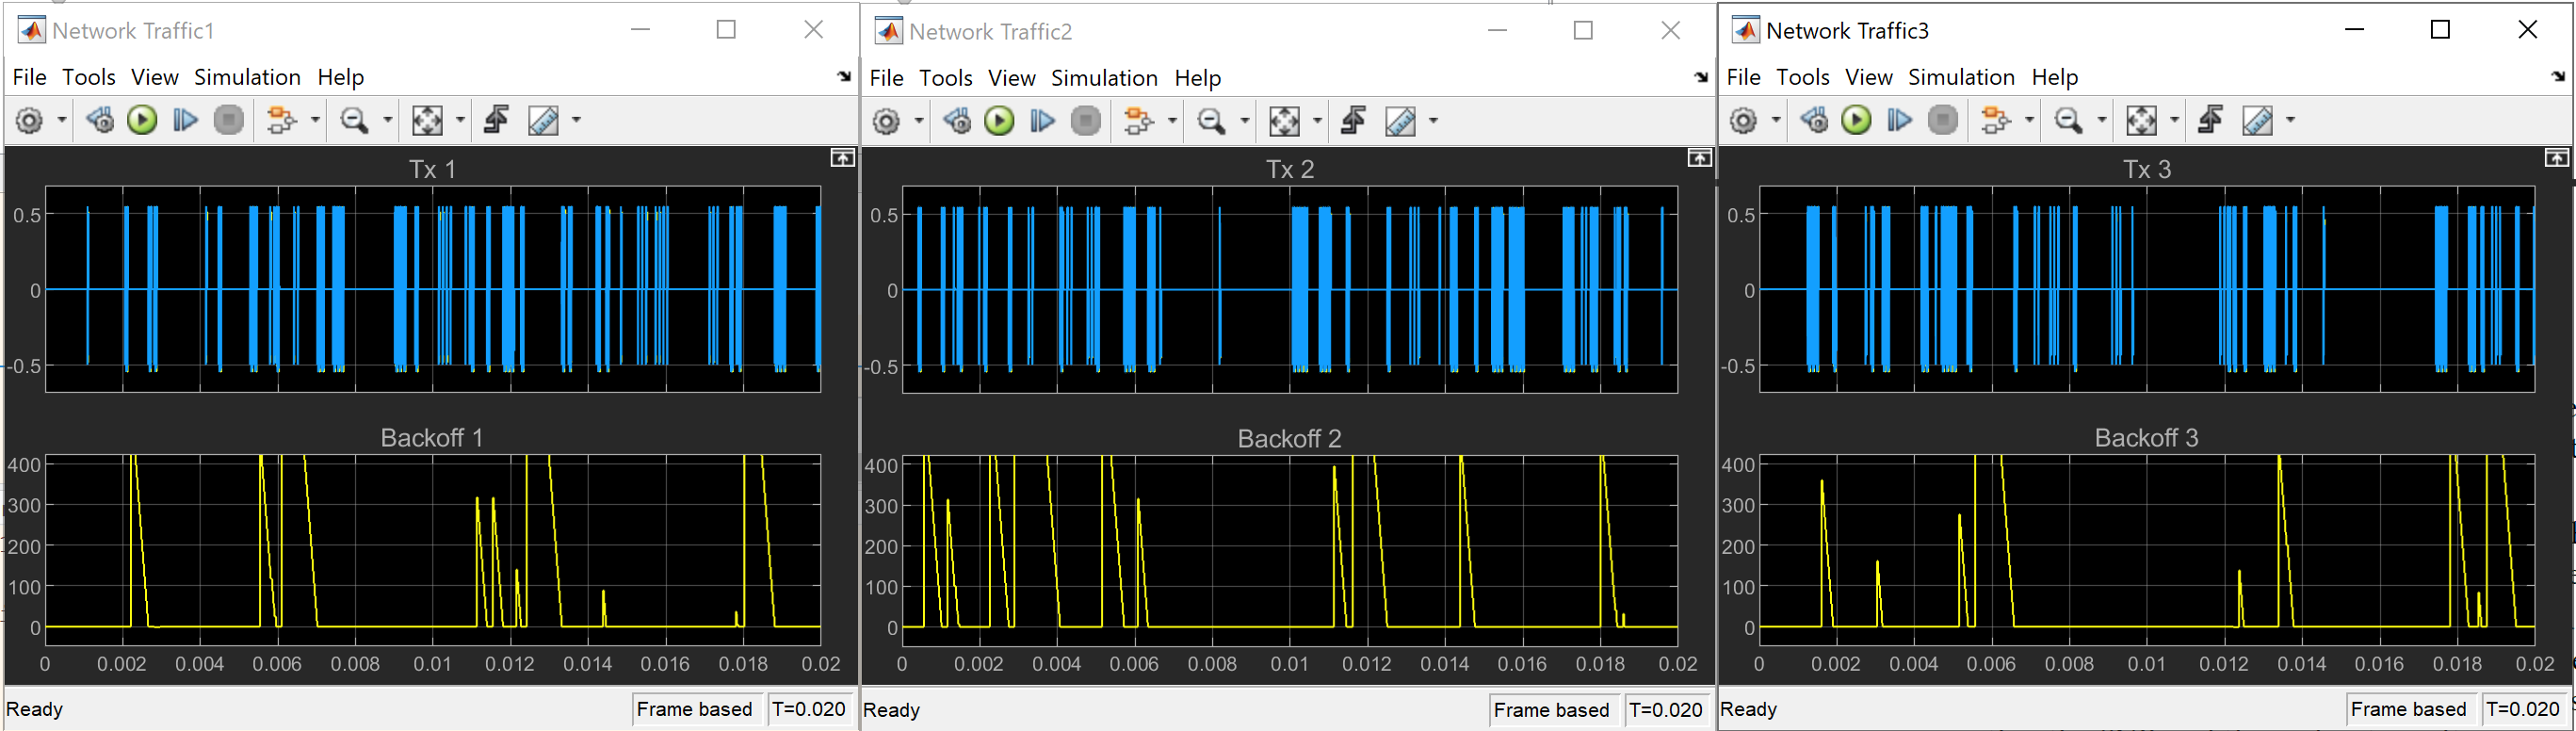
\includegraphics[width=\maxwidth{50.17561465127948em}]{image_0}
\end{flushleft}
\end{par}

\begin{par}
\begin{flushleft}
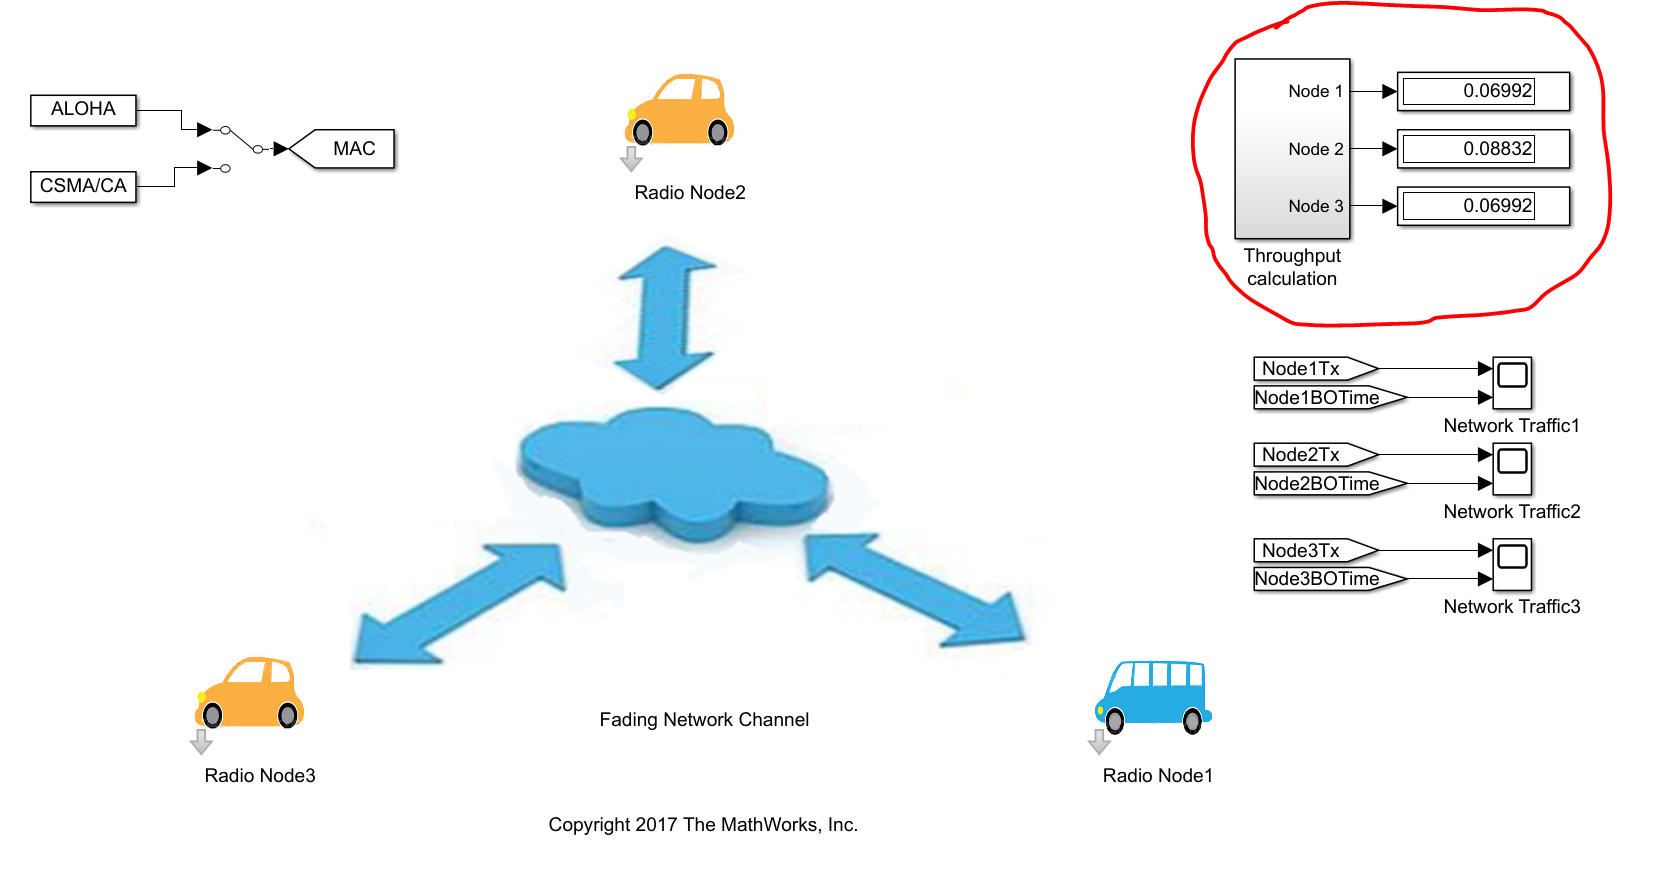
\includegraphics[width=\maxwidth{50.17561465127948em}]{image_1}
\end{flushleft}
\end{par}

\matlabtitle{P3-C-2}

\begin{par}
\begin{flushleft}
Using the CSMA/CA model:
\end{flushleft}
\end{par}

\begin{par}
\begin{flushleft}
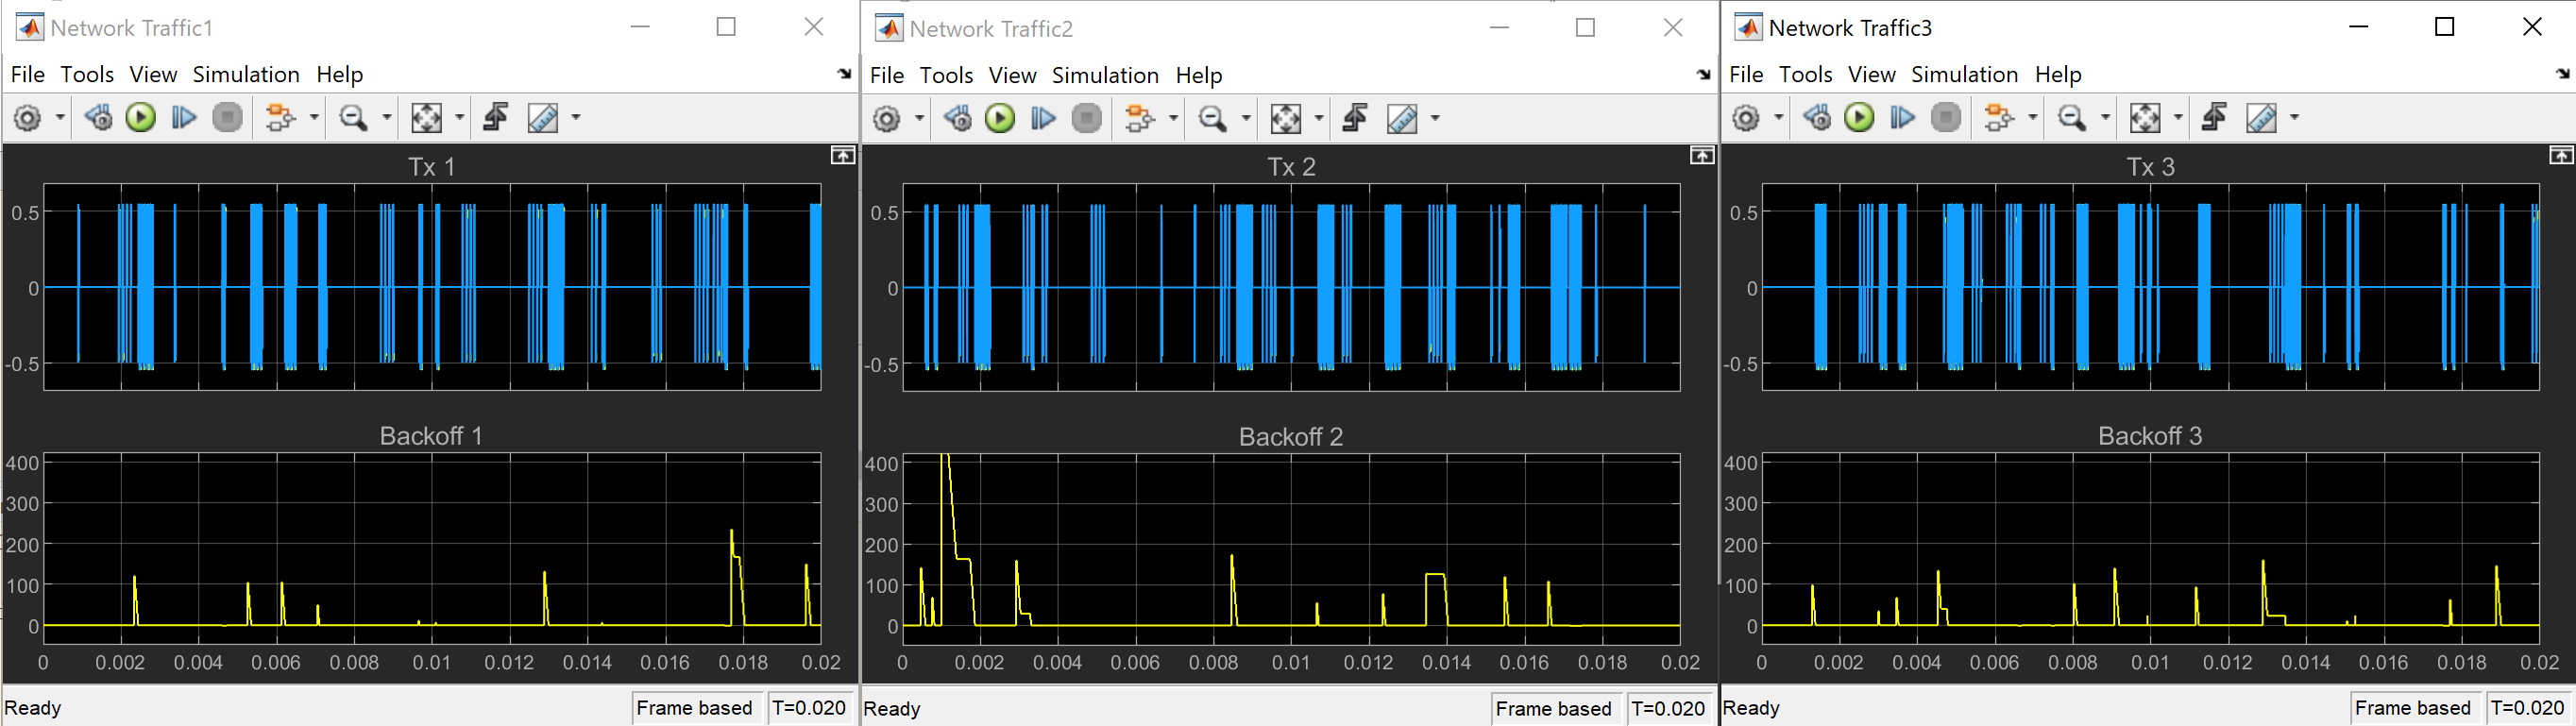
\includegraphics[width=\maxwidth{50.17561465127948em}]{image_2}
\end{flushleft}
\end{par}

\begin{par}
\begin{flushleft}
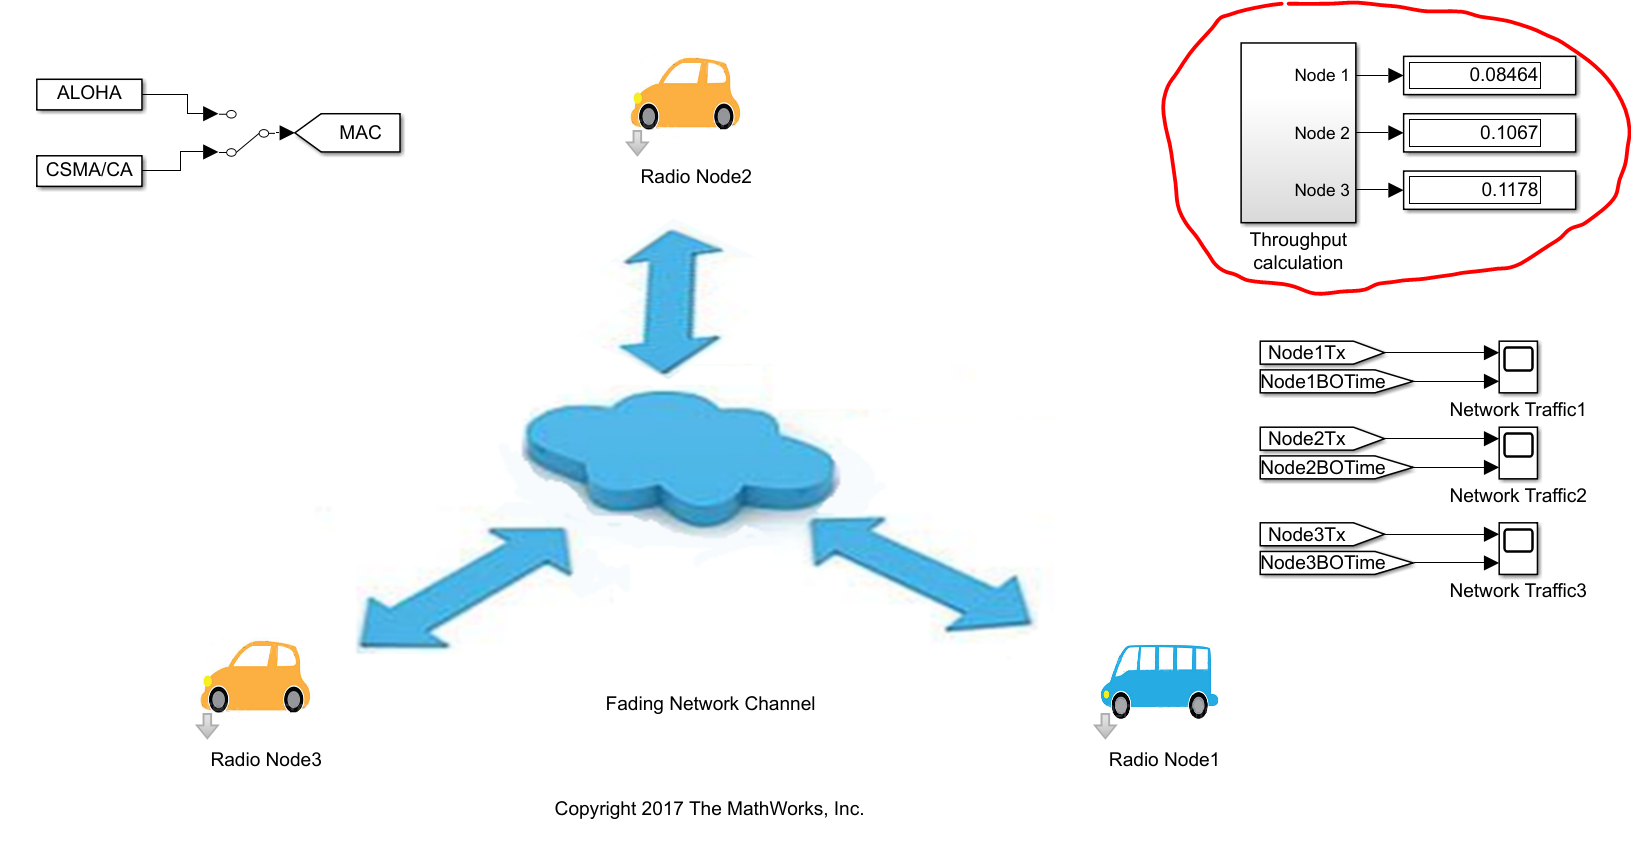
\includegraphics[width=\maxwidth{50.17561465127948em}]{image_3}
\end{flushleft}
\end{par}

\matlabtitle{P3-C-3}

\begin{par}
\begin{flushleft}
Modifying the SNR of white noise to 22 Eb/No and running the simulation again:
\end{flushleft}
\end{par}

\begin{par}
\begin{flushleft}
Using the ALOHA model:
\end{flushleft}
\end{par}

\begin{par}
\begin{flushleft}
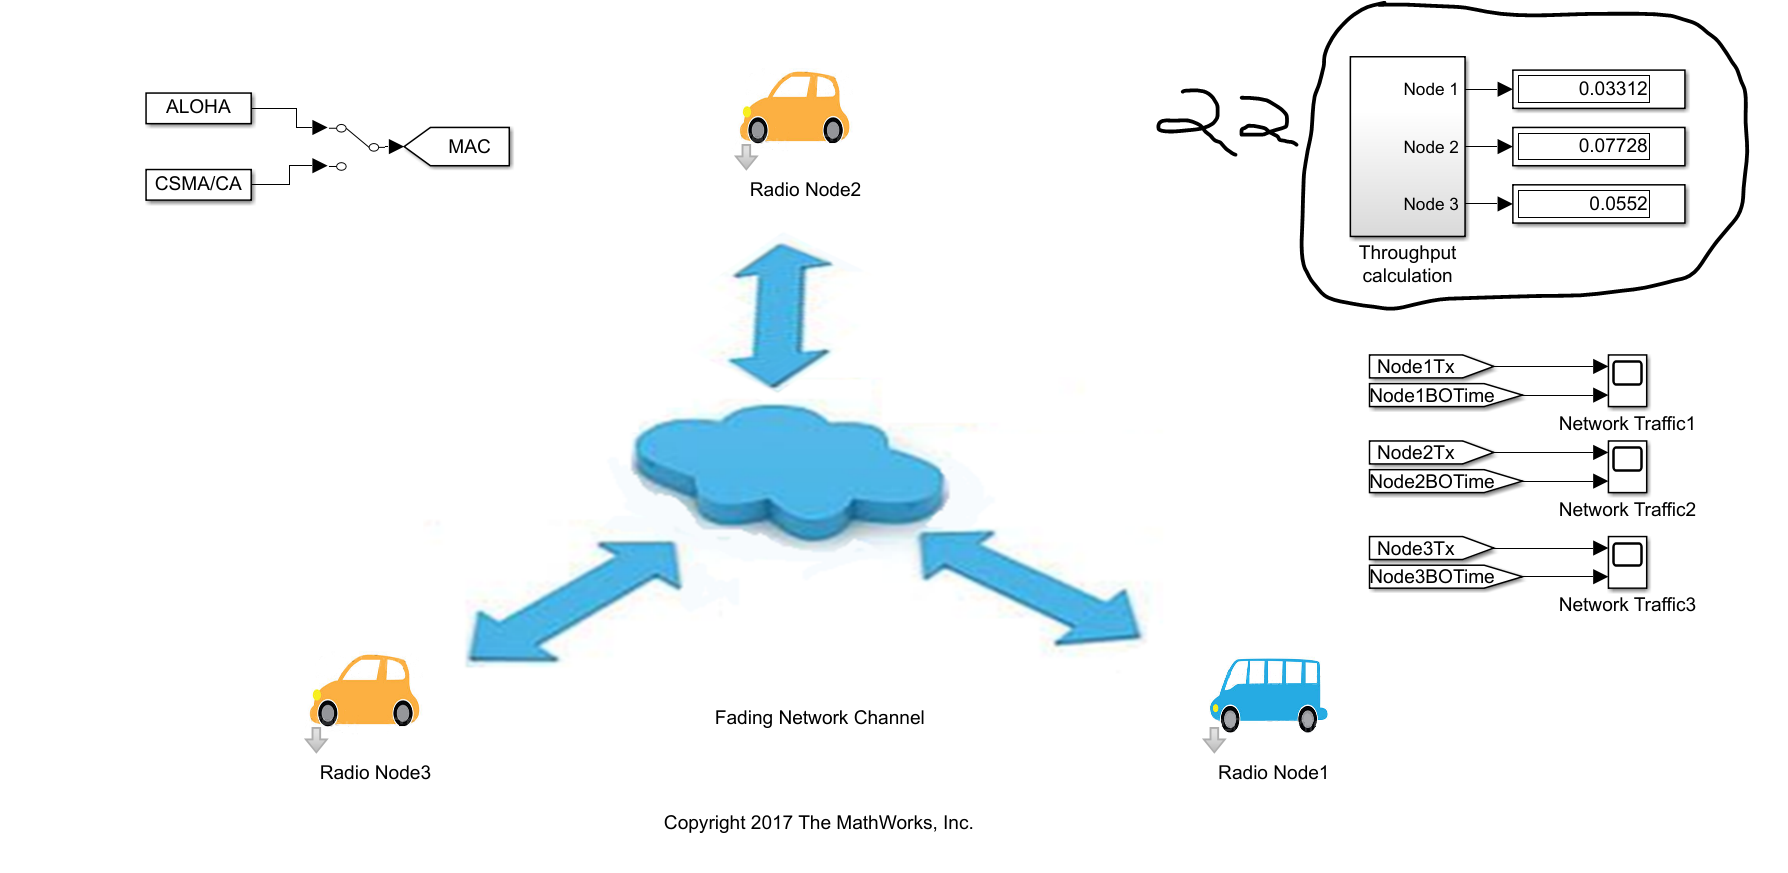
\includegraphics[width=\maxwidth{50.17561465127948em}]{image_4}
\end{flushleft}
\end{par}

\begin{par}
\begin{flushleft}
Using the CSMA/CA model:
\end{flushleft}
\end{par}

\begin{par}
\begin{flushleft}
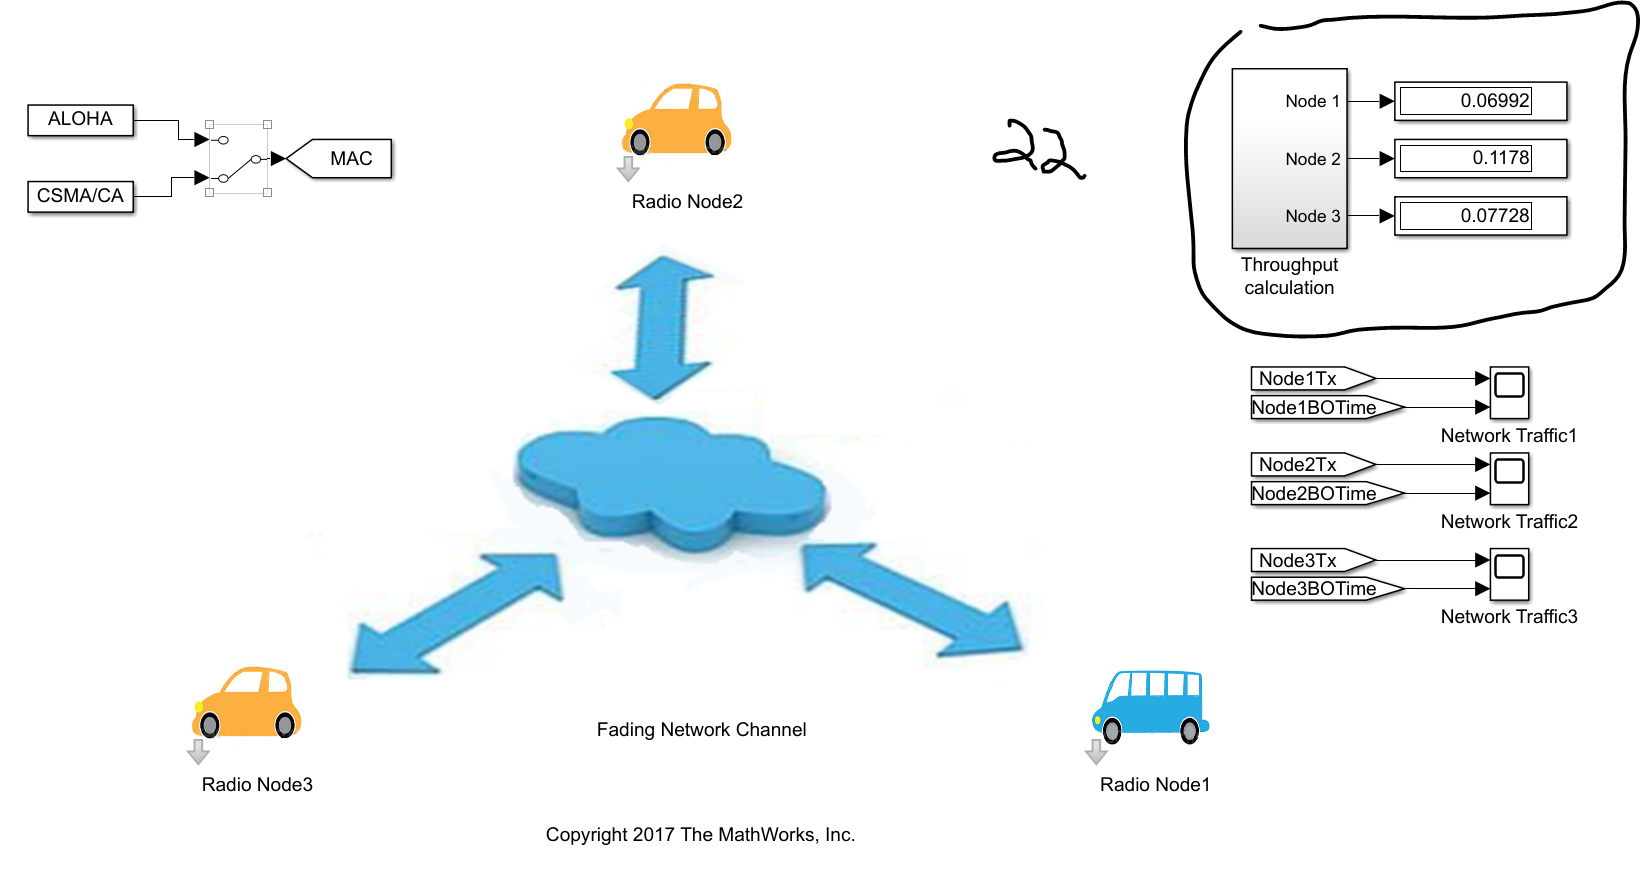
\includegraphics[width=\maxwidth{50.17561465127948em}]{image_5}
\end{flushleft}
\end{par}

\matlabtitle{P3-C-4}

\begin{par}
\begin{flushleft}
We observed a decreased throughput. This is expected because a lower signal-to-noise ratio means either the tranmitting signal has less power or the noise is stronger, and both will decrease the efficiency of tranmission. 
\end{flushleft}
\end{par}


\matlabtitle{P4}

\begin{par}
\begin{flushleft}
Two retranmission-based error controlling mechanism is stop-and-wait ARQ and continuous ARQ. 
\end{flushleft}
\end{par}

\begin{par}
\begin{flushleft}
With stop-and-wait ARQ, the receiver receives frame and sends ACK if no error or NAK if error. If NAK, sender will resend data. If no ACK or NAK, sender retranmits frame after timeout. If no ACK, sender resends data and receiver sends ACK and deletes duplicate frame.
\end{flushleft}
\end{par}

\begin{par}
\begin{flushleft}
With continuous ARQ, sender does not wait for ACKS before sending more data. Slidingwindow is the number of frames allowed to be unacknolowedged by receiver, and the number of frames that be sent depends on window size, which is agreed upon by sender and receiver at the beginning. 
\end{flushleft}
\end{par}


\matlabtitle{P5-A}

\begin{matlabcode}
question();
hostBits = ceil(log2(100))
\end{matlabcode}
\begin{matlaboutput}
hostBits = 7
\end{matlaboutput}

\begin{par}
\begin{flushleft}
Since the minimum of seven bits are needed, class A,B,and C can would all suffice. However, to acquire longer network ID bits availibilities, class C is enough.
\end{flushleft}
\end{par}

\matlabtitle{P5-B}

\begin{par}
\begin{flushleft}
If CIDR is used, then we can use the remaining bits as CIDR N bits:
\end{flushleft}
\end{par}

\begin{matlabcode}
cidrBits = 32-hostBits;
answer(cidrBits,"");
\end{matlabcode}
\begin{matlaboutput}
 ANSWER: 25 [] 
\end{matlaboutput}


\matlabtitle{P6}

\begin{par}
\begin{flushleft}
Computer\#1→Interface1@Gateway:
\end{flushleft}
\end{par}

\begin{itemize}
\setlength{\itemsep}{-1ex}
   \item{\begin{flushleft} Source IP Address: IP1 \end{flushleft}}
   \item{\begin{flushleft} Destination IP Address: IP2 \end{flushleft}}
   \item{\begin{flushleft} MAC Address: MAC3 \end{flushleft}}
\end{itemize}

\begin{par}
\begin{flushleft}
Interface2@Gateway→Computer\#2:
\end{flushleft}
\end{par}

\begin{itemize}
\setlength{\itemsep}{-1ex}
   \item{\begin{flushleft} Source IP Address: IP1 \end{flushleft}}
   \item{\begin{flushleft} Destination IP Address: IP2 \end{flushleft}}
   \item{\begin{flushleft} MAC Address: MAC2 \end{flushleft}}
\end{itemize}


\matlabtitle{P7-A}

\begin{par}
\begin{flushleft}
Subnetting help organize IP address within networks and organizations and allows organizations to distribute pool of IP addresses in subnets (depending upon organization structure).
\end{flushleft}
\end{par}

\matlabtitle{P7-B}

\begin{matlabcode}
subnetMask=[255,255,254,0];
subnetMask = dec2bin(subnetMask);
subnetMask = reshape(subnetMask',1,[])
\end{matlabcode}
\begin{matlaboutput}
subnetMask = '11111111111111111111111000000000'
\end{matlaboutput}
\begin{matlabcode}
subnetMaskBits = sum(subnetMask=='1');
hostIdBits = size(subnetMask,2)-subnetMaskBits;
answer(hostIdBits,"");
\end{matlabcode}
\begin{matlaboutput}
 ANSWER: 9 [] 
\end{matlaboutput}

\begin{par}
\begin{flushleft}
From the binary format of subnet mask, we can see the last 9 bits are not used for subnet address, which means the host ID can contain 9 bits.
\end{flushleft}
\end{par}

\matlabtitle{P7-C}

\begin{matlabcode}
netIdBits = 16;
subnetIdBits = subnetMaskBits-netIdBits;
answer(subnetIdBits,"");
\end{matlabcode}
\begin{matlaboutput}
 ANSWER: 7 [] 
\end{matlaboutput}

\matlabtitle{P7-D}

\begin{matlabcode}
maxSubnet = power(2,subnetIdBits);
answer(maxSubnet,"");
\end{matlabcode}
\begin{matlaboutput}
 ANSWER: 128 [] 
\end{matlaboutput}

\matlabtitle{P7-E}

\begin{matlabcode}
ip = [192,168,255,40];
ip = dec2bin(ip);
ip = reshape(ip',1,[]);
maskedIp = char((ip=='1'&subnetMask=='1')+'0')
\end{matlabcode}
\begin{matlaboutput}
maskedIp = '11000000101010001111111000000000'
\end{matlaboutput}
\begin{matlabcode}
maskedIp = reshape(maskedIp,log2(256),[])';
maskedIp = bin2dec(maskedIp)'
\end{matlabcode}
\begin{matlaboutput}
maskedIp = 1x4    
   192   168   254     0

\end{matlaboutput}


\matlabtitle{P8}

\begin{par}
\begin{flushleft}
The shortage of IPv4 is handled by Network Address Translation or IPv6. In NAT, some IP addresses are reused as a small pool of IP addresses to serve a large number of computers, which will not be globally unique. IPv6 on the other hand simply defines a new standard in RFC2460 which expands source and destination address fields from 32 bits to 128 bits. 
\end{flushleft}
\end{par}


\begin{matlabcode}
function table_out = transmit(dest,port,table_in)
%For Problem 2
    table_out = table_in;
    if(isKey(table_in,dest))
        fprintf("Cache hit from table.\n");
    else
        fprintf("Cache miss from table, create pair {%s,%s}.\n",dest,port);
        table_out(dest) = port;
    end
    disp([table_out.keys',table_out.values']);
end
\end{matlabcode}

\end{document}
